
\chapter{راه‌حل پیشنهادی}

مساله‌ی بیان شده به صورت \lr{ILP}
مدل‌سازی می‌شود.
در \cite{Eramo2016}
مساله‌ی جایگذاری \lr{SFC}ها با هدف حداکثرسازی تعداد درخواست‌های پذیرفته شده
به صورت \lr{ILP} مدل‌سازی شده و اثبات شده است که مساله‌ی حاضر \lr{NP-Hard} می‌باشد.
مساله‌ای که در اینجا مدل‌سازی می‌شود از آن مساله پیچیده‌تر می‌باشد زیرا در نظر گرفتن \lr{VNFM}ها را نیز شامل می‌شود.
برای این مساله می‌توان
یک راه حل مکاشفه‌ای با زمان چند جمله‌ای
پیشنهاد داد.

\section{الگوریتم مکاشفه‌ای}

مساله از دو قسمت تشکیل شده است. قسمت اول مساله‌ی جایگذاری لینک‌ها و نمونه‌ها می‌باشد
و قسمت دوم جایگذاری
\lr{VNFM}
برای زنجیره است.
برای قسمت اول راه‌حل‌های مکاشفه‌ای زیادی ارائه شده است که ما در اینجا
از راه‌حل \cite{Bari2015} استفاده می‌کنیم.
در این راه حل برای قرارگیری هر زنجیره یک گراف چند گامی شکل می‌گیرد.
هر گام این گراف نماینده یک نمونه از زنجیره است که می‌بایست قرار گیرد.
در نظر داشته باشید که مساله‌ی اصلی و راه‌حل بهینه می‌توانند روی ورودی مشابه با \lr{VNF-FG}
فعالیت کنند و این در حالی است که راه‌حل پیشنهادی تنها می‌تواند پذیرا زنجیره‌ها باشد.
در هر گام از این گراف مجموعه‌ای از نودهای فیزیکی امکان پذیر شکل می‌گیرد.
با توجه به وضعیت مسیریابی این مجموعه با مجموعه بعدی نود فیزیکی برای نمونه مورد نظر از زنجیره انتخاب می‌شود.

\begin{figure}[h]
\center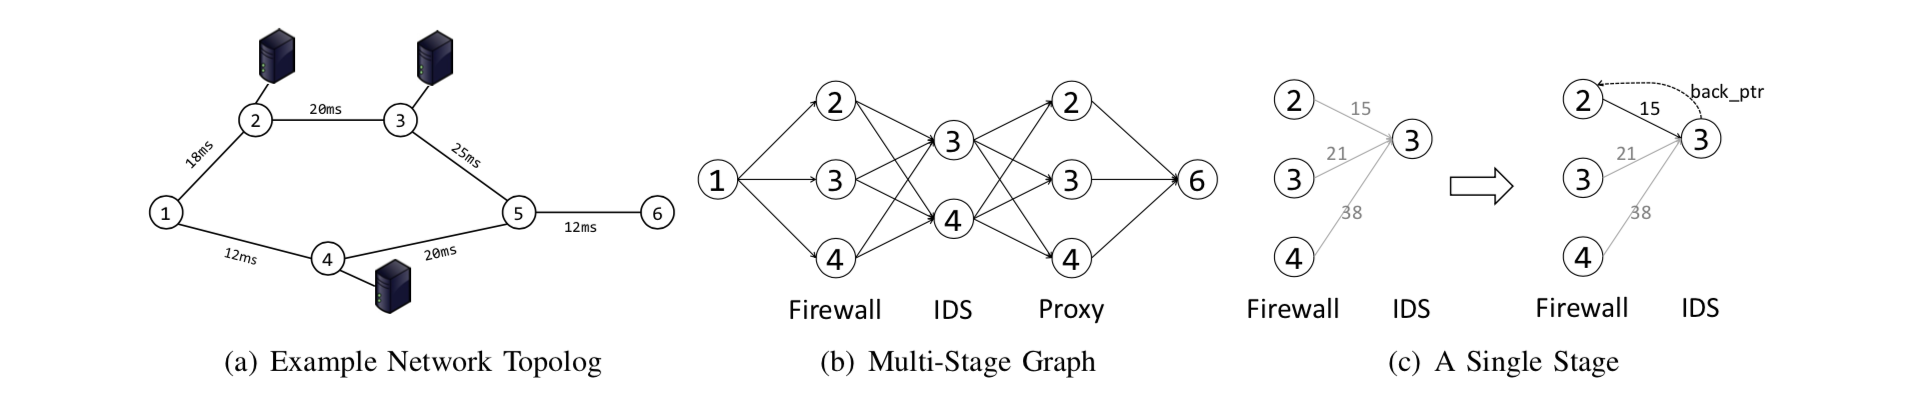
\includegraphics[scale=.45]{images/bari}
\caption{مدل‌سازی با گراف چندگامی \cite{Bari2015}}
\label{fig.5}
\end{figure}

منظور از وضعیت مسیریابی به شرح زیر است. برای هر یک از گام‌ها از الگوریتم جستجوی اول سطح یا
\lr{BFS}
استفاده می‌کنیم
و به این ترتیب مسیرهای فیزیکی که می‌توان از آن‌ها برای جایابی لینک مجازی استفاده کرد پیدا می‌کنیم.
از این بین گره‌ای که مسیرهای فیزیکی امکان‌پذیر بیشتری دارد انتخاب می‌گردد.
با این روش مجموعه امکان‌پذیر گام بعدی بزرگتر می‌شود و امکان حذف زنجیره به دلیل نبود مسیر فیزیکی
برای جایابی لینک مجازی کمتر می‌گردد.

در ادامه یک گام به این الگوریتم اضافه می‌کنیم که در آن برای هر زنجیره بعد از قرارگرفتن یک
\lr{VNFM}
تخصیص می‌دهیم. برای اینکار مجموعه‌ای امکان‌پذیر از نودهای فیزیکی را انتخاب می‌کنیم
و سعی می‌کنیم از بین آن‌ها انتخاب کنیم. در روند این انتخاب از اصول زیر پیروی می‌کنیم:

\begin{itemize}
    \item اولویت با نود فیزیکی است که روی آن \lr{VNFM} با ظرفیت خالی وجود دارد.
    \item از بین نودهایی که ظرفیت خالی دارند اولویت با نودی است که منابع پردازشی بیشتری دارد.
\end{itemize}

از آنجایی که مساله‌ی طرح شده به صورت آفلاین می‌باشد می‌توان با بررسی ورودی‌های الگوریتم کارآیی آن را بهبود داد.
برای این منظور زنجیره‌های ورودی را برحسب اندازه‌ی آن‌ها مرتب می‌کنیم.
در این مرتب‌سازی تلاش می‌شود که زنجیره‌های بزرگتر که سود بیشتری دارند زودتر جایابی شوند.
به این ترتیب برای زنجیره‌هایی که سود بیشتری دارند منابع بیشتری در اختیار الگوریتم قرار دارد.

\subsection{شبه کد}

شبه کد سطح بالای الگوریتم پیشنهادی به شرح زیر می‌باشد:

\begin{latin}
    \begin{verbatim}
          sorts.Slice(chains, func (i, j int) {
            return len(chains[i]) > len(chains[j])
          })
          
          for i := 0; i < len(chains); i++ {
            chain := chains[i]
            var feasibleSet []Node
            for i := 0; i < len(chain); i++ {
              if i == 0 {
                feasibleSet = feasibleSetForInstance(i, nil)
              } else {
                selectedNode := nodesWithMaximumReachableNodes(
                  feasibleSet(i - 1))[0]
                if selectedNode == nil {
                  break
                }
                feasibleSetForInstance(i, selectedNode)
              }
            }
            feasibleManagers := feasibleManagerforChain(chain)
            selectedManager = vnfmWithMoreAvailableResources(
              vnfmWithEmptyCapacity(
                feasibleManagers))[0]
            if selectedManager == nil {
              break
            }
          }
    \end{verbatim}
\end{latin}

در اولین گام زنجیره‌ها بر اساس قیمت‌شان مرتب می‌شوند.
در نظر داشته باشید که قیمت هر زنجیره ارتباط مستقیمی با تعداد نمونه‌های آن دارد
بنابراین با این روش در ابتدا که شبکه زیرساخت خالی است زنجیره‌هایی با ابعاد بزرگتر و سود بیشتر جایگذاری می‌شوند.
در گام بعدی زنجیره‌ها به ترتیب پیمایش  شده و سعی در جایگذاری آن‌ها می‌شود.
برای جایگذاری هر زنجیره تمامی نمونه‌های آن به ترتیب پیمایش می‌شوند.
برای هر نمونه ابتدا از مجموعه امکان‌پذیر نمونه‌ی قبلی یک نود فیزیکی انتخاب می‌شود که این انتخاب بر اساس تعداد نودهای قابل دسترس از هر نود صورت می‌پذیرد و
در ادامه یک مجموعه امکان‌پذیر از نودهای فیزیکی انتخاب می‌شود که این انتخاب بر اساس گام قبلی صورت می‌گیرد.
در نظر داشته باشید که انتخاب نودی که نودهای بیشتری از آن قابل دسترس می‌باشند احتمال خالی شدن مجموعه امکان‌پذیر در گام‌های بعدی را کاهش می‌دهد.

در نهایت بعد از اینکه تمامی نمونه‌های زنجیره جایگذاری شدند \lr{VNFM} بر اساس معیارهایی که پیشتر شرح داده شد انتخاب می‌شود.

\subsection{پیچیدگی}

الگوریتم پیشنهادی برای \(n\) زنجیره با یک مرحله مرتب‌سازی با زمان \(O(nlogn)\) آغاز می‌شود.
در ادامه جایگذاری هر زنجیره به تعداد نمونه‌های آن زنجیره الگوریتم \lr{BFS} را اجرا می‌کند.
تعداد نمونه‌های هر زنجیره عددی مشخص و کوچک است بنابراین می‌توان از آن به عنوان یک ثابت صرف نظر کرد
اما زمان اجرای الگوریتم \lr{BFS} به اندازه‌ی یال‌های شبکه زیرساخت می‌باشد
پس در بدترین حالت (زمانی که مجموعه‌ی امکان‌پدذیر همه‌ی نودهای شبکه‌ی زیرساخت را در بر دارد)‌ زمان اجرا از
\(O(VE)\)
می‌باشد و در نهایت الگوریتم از زمان اجرای زیر پیروی می‌کند:

$$
O(nVE)
$$

\subsection{زمان اجرا}

نکته‌ای که نیاز به توجه دارد زمان حل است. در دنیای واقعی تغییرات زنجیره‌ها در دیتاسنتر نیاز به اعمال در بازه‌های زمانی کوتاهی دارد که
حتی ممکن زمان ۱۵ دقیقه هم برای آن زیاد باشد.
به همین منظور در ادامه بهبودی برای زمان اجرا ارائه می‌کنیم.

الگوریتم \cite{Bari2015} در هر گام نود فیزیکی گام قبلی را نهایی کرده و مجموعه امکان‌پذیر این گام را مشخص می‌کند.
این امر نیاز به اجرای چند مرحله الگوریتم مسیریابی اول سطح یا \lr{BFS} دارد که
می‌بایست بر روی کل توپولوژی اجرا شود.
برای توپولوژی‌هایی که تعداد نودهای آن‌ها زیاد است زمان زیادی برای این عملیات لازم است.
برای کاهش این زمان می‌توان درصد مشخصی از زنجیره‌ها را با روش \lr{first-fit} جایگذاری کرده و زمان اجرا الگوریتم را کاهش داد.

\section{جمع‌بندی}

در این فصل الگوریتم پیشنهادی برای جایگذاری زنجیره‌ها و منابع مدیریتی آن‌ها پیشنهاد شد.
این الگوریتم از الگوریتم \cite{Bari2015}
به عنوان الگوریتم پایه استفاده می‌کند و با مرتب‌سازی اولیه زنجیره‌ها
و جایگذاری \lr{fisrt-fit}
تعدادی از زنجیره‌ها کارآیی و زمان اجرا الگوریتم را بهبود می‌دهد.
برای جایگذاری منابع مدیریتی سعی می‌شود با استفاده از گواهی‌های مشترک برای زنجیره‌ها
هزینه‌ی گواهی را که تاثیر مستقیمی بر تابع هدف دارد کاهش داد.

به صورت کلی الگوریتم پیشنهادی بهبودهای زیر را نسبت به الگوریتم \cite{Bari2015} ارائه می‌کند:

\begin{itemize}
  \item
  با مرتب‌سازی ورودی بر اساس قیمت زنجیره‌ها که ارتباط مستقیمی با تعداد نمونه‌های آن‌ها دارد
  سعی می‌کند سود بیشتری را از نگاشت نمونه‌ها حاصل کند.
  \item
  جایگذاری نسبت مشخصی از زنجیره‌ها با الگوریتم \lr{first-fit} که باعث صرفه‌جویی در زمان اجرای الگوریتم می‌شود.
  در نظر داشته باشید که مساله فرض می‌کند شبکه زیرساخت در ابتدا خالی است بنابراین برای جایگذاری زنجیره‌های اولیه نیاز به اخذ تصمیمات پیچیده نداریم.
\end{itemize}